\documentclass[24pt,aspectratio=169]{beamer}
\graphicspath{{Images/}{./}} % Specifies where to look for included images (trailing slash required)
\usetheme{metropolis}

\usepackage[spanish]{babel} % Cargar el paquete babel con la opción spanish
\usepackage[utf8]{inputenc} % Asegurar la codificación UTF-8
\usepackage{appendixnumberbeamer}
\usepackage{booktabs}
\usepackage[scale=2]{ccicons}
\usepackage{pgfplots}
\usepackage{xcolor} % Cargar el paquete xcolor
\usepackage{xspace}
\usepackage[round]{natbib}
\usepackage{ragged2e}
\usepackage{bbding} %palomitas checkmark
\usepgfplotslibrary{dateplot}

\usepackage[ruled,vlined]{algorithm2e}
\usepackage{dirtree}
\usepackage{xcolor}

\usepackage{rotating}
\usepackage{tikz}

\usepackage{array} % needed for \arraybackslash
\usepackage{graphicx}
\usepackage{adjustbox} % for \adjincludegraphics

\usepackage{subcaption}
\usepackage{bibentry}
%\bibliographystyle{apalike}
\usepackage{chngcntr}
\usepackage{lipsum}% http://ctan.org/pkg/lipsum
\usepackage{hanging}% http://ctan.org/pkg/hanging

\usepackage{xcolor,colortbl}
\usepackage{multirow}

\usepackage{animate}
\usepackage{multicol}
\usepackage{tabularx,booktabs}
\usepackage{forloop}
\usepackage{ragged2e}

\usepackage{bbding} %palomitas checkmark
\usepackage{pifont}
\usepackage{lipsum,tabularx}

\usepackage{tikz}
\usetikzlibrary{arrows.meta, positioning, shapes.multipart}

\usepackage{tikz}
\usetikzlibrary{shapes,arrows}
\usepackage{amsmath,bm,times}

\usepackage{enumitem}

%\usepackage{circuitikz}
\usepackage{longtable}

\usepackage{progressbar}

\usepackage{pgfgantt}

\newcommand{\mx}[1]{\mathbf{\bm{#1}}} % Matrix command
\newcommand{\vc}[1]{\mathbf{\bm{#1}}} % Vector command

%\usepackage{annotate-equations}
\newcounter{loopcntr}

\definecolor{verde_cinves}{HTML}{009383} % Color de primer plano (foreground) de la barra de progreso
\definecolor{azulrey_cinves}{HTML}{005179} % Color de primer plano (foreground) de la barra de progreso
\definecolor{amarillo_cinves}{HTML}{FFDA72} % Color de primer plano (foreground) de la barra de progreso

\newcommand{\themename}{\textbf{\textsc{metropolis}}\xspace}

%separador titulo inicio
\setbeamercolor{title separator}{use=structure,fg=azulrey_cinves!50, bg=azulrey_cinves!10}

%barra que anuncia el nombre de la seccion
\setbeamercolor{progress bar in section page}{use=structure,fg=azulrey_cinves!100, bg=azulrey_cinves!10}

%barra de titulo en cada section page
\setbeamercolor{frametitle}{use=structure,fg=azulrey_cinves!5, bg=azulrey_cinves!100}

\title{\large{Estrategias para la exploración coordinada multi-VANT}}
%\subtitle{A modern beamer theme}
\author{Tesista: Luis Alberto Ballado Aradias\\[\baselineskip]
  \small{{Asesores:} 
    \and\\Dr. José Gabriel Ramírez-Torres
    \and\\Dr. Eduardo Rodriguez-Tello\\ }
}
\date{\today}
\institute{Centro de Investigación y de Estudios Avanzados - Unidad Tamaulipas}
\titlegraphic{\hfill
\includegraphics[height=1.5cm]{cinvestav_negro}}

\newcommand{\rpt}[2][1]{%
  \forloop{loopcntr}{0}{\value{loopcntr}<#1}{#2}%
}

\newcommand{\on}[1][1]{
  \forloop{loopcntr}{0}{\value{loopcntr}<#1}{&\cellcolor{lightgray}}
}
\newcommand{\onok}[1][1]{
  \forloop{loopcntr}{0}{\value{loopcntr}<#1}{&\cellcolor{green}}
}
\newcommand{\ondelay}[1][1]{
  \forloop{loopcntr}{0}{\value{loopcntr}<#1}{&\cellcolor{red!60}}
}
\newcommand{\off}[1][1]{
  \forloop{loopcntr}{0}{\value{loopcntr}<#1}{&\cellcolor{white}}
}

\addtolength{\textheight}{90pt}

\newcommand{\I}{\mathbb{I}}
\newcommand{\K}{\mathbb{K}}
\newcommand{\N}{\mathbb{N}}
\newcommand{\Q}{\mathbb{Q}}
\newcommand{\R}{\mathbb{R}}
\newcommand{\Z}{\mathbb{Z}}

\newcommand{\specialcell}[2][c]{%
  \begin{tabular}[#1]{@{}c@{}}#2\end{tabular}}

% Definir comandos para checkmark y cross
\newcommand{\cmark}{{\color{green}\ding{51}}} % Checkmark en verde
\newcommand{\xmark}{{\color{red}\ding{55}}}   % Cross en rojo

%Used to draw gantt charts, which I will use for the calendar.
%Let's define some awesome new ganttchart elements:
\newganttchartelement{orangebar}{
    orangebar/.style={
        inner sep=0pt,
        draw=red!66!black,
        very thick,
        top color=white,
        bottom color=orange!80
    },
    orangebar label font=\slshape,
    orangebar left shift=.1,
    orangebar right shift=-.1
}

\newganttchartelement{bluebar}{
    bluebar/.style={
        inner sep=0pt,
        draw=purple!44!black,
        very thick,
        top color=white,
        bottom color=blue!80
    },
    bluebar label font=\slshape,
    bluebar left shift=.1,
    bluebar right shift=-.1
}

\newganttchartelement{greenbar}{
    greenbar/.style={
        inner sep=0pt,
        draw=green!50!black,
        very thick,
        top color=white,
        bottom color=green!80
    },
    greenbar label font=\slshape,
    greenbar left shift=.1,
    greenbar right shift=-.1
}

\begin{document}

\maketitle

\begin{frame}{Contenido}
  \setbeamertemplate{section in toc}[sections numbered]
  \tableofcontents[hideallsubsections]
\end{frame}

\section{Introducción}

\begin{frame}[fragile]{Antecedentes}
  \bigskip % Vertical whitespace
  \centering
  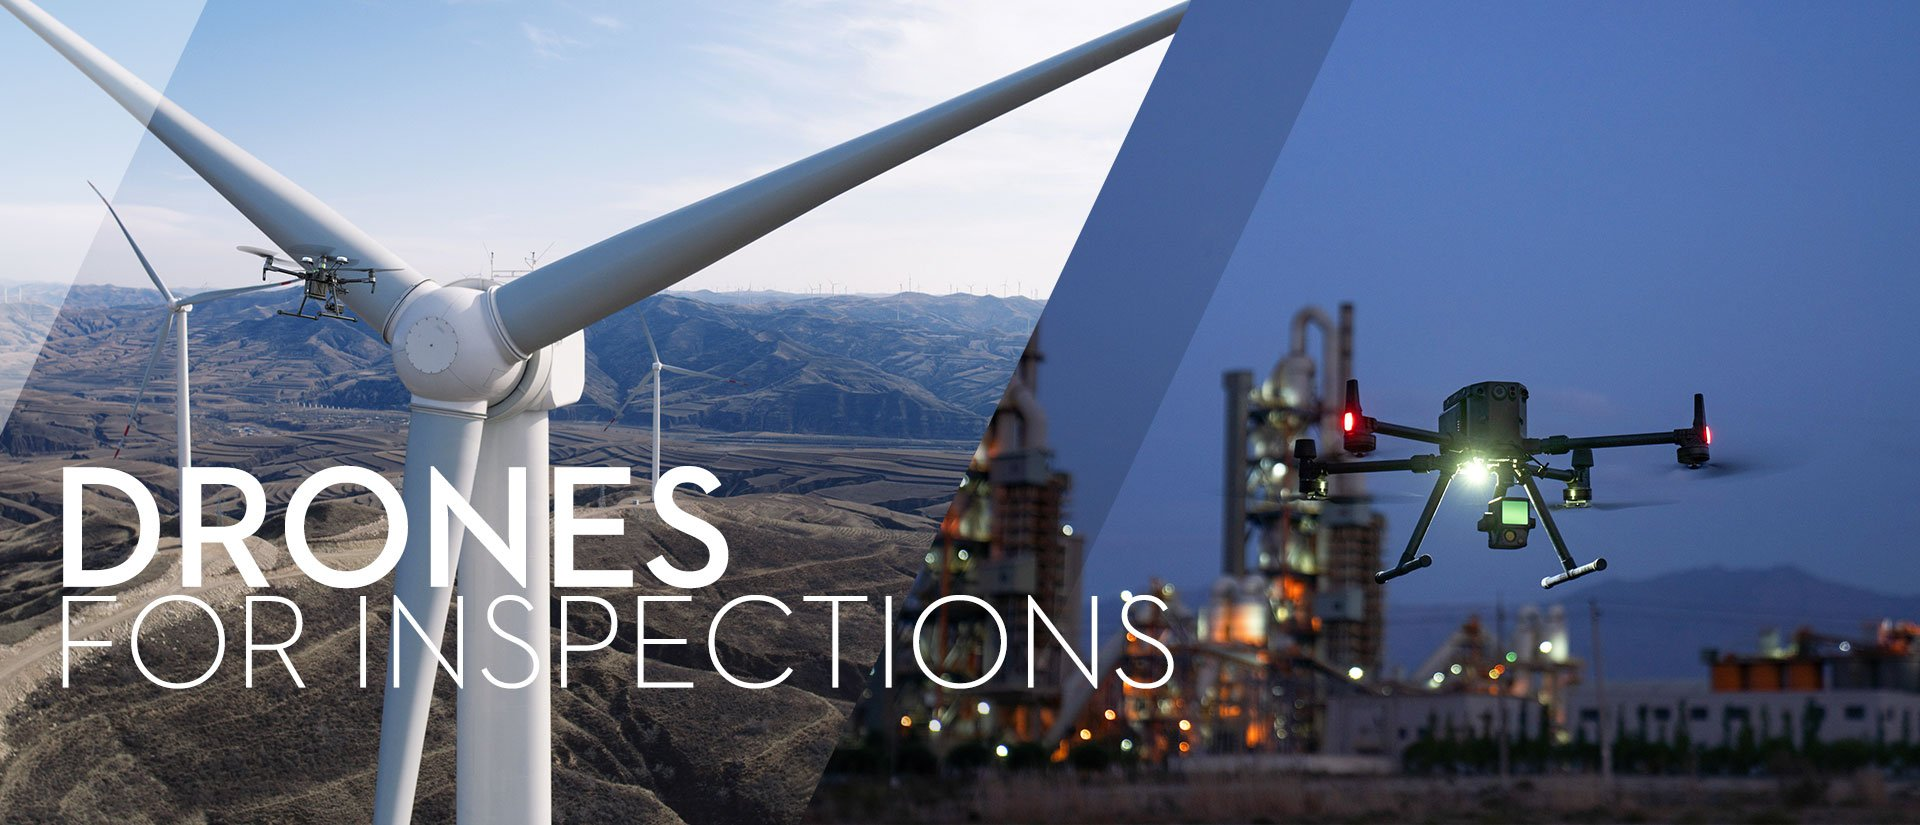
\includegraphics[width=0.45\textwidth,height=0.35\textheight]{DJI_B1}$^\dag$
  \hfil
  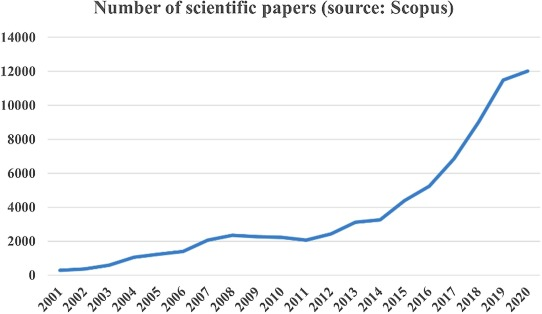
\includegraphics[width=0.45\textwidth,height=0.35\textheight]{survey_chart.jpg}\footnotemark
  %\vspace{1pt}\\
  
  \begin{itemize}
  \item \textbf{UAV} {\tiny(\textit{Vehículo Aéreo No Tripulado - VANT})}  $\implies$ \textbf{UAS} {\tiny(\textit{Sistemas Aéreos No Tripulado - SANT})}
  \item \textbf{Aplicaciones} en lugares inaccesibles o peligrosos.
  \item \textbf{Múltiples VANT} pueden aumentar la confianza del sistema.
  \item \textbf{Limitaciones} en carga, procesamiento y batería \small{influyen en el tiempo de vuelo.}
  \end{itemize}
  
  \tiny{
    \footnotetext{UAV in the advent of the twenties: Where we stand and what is next [\cite{Nex2022}]}
  }
\end{frame}

\begin{frame}{Antecedentes}

  %Exploración es una tarea fundamental en robots autónomos.\\
  %El objetivo es crear un mapa de un ambiente desconocido.\\
  %\bigskip % Vertical whitespace
  \centering
  \bigskip % Vertical whitespace
  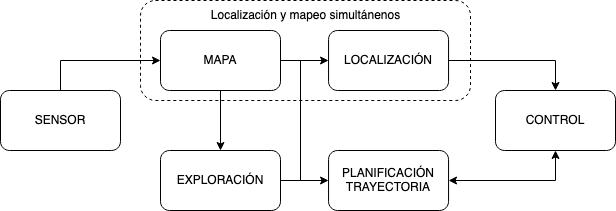
\includegraphics[width=9cm]{exploracion}\\
  
  \begin{itemize}
  \item \textbf{Sensar}
  \item \textbf{Creación Mapa} 
  \item \textbf{Localización en Mapa}
  \item \textbf{\textcolor{blue}{Exploración}} (Aumentar la base de conocimiento del mapa)
  \item \textbf{\textcolor{blue}{Planificación trayectoria}} (Trayectorias hacia nuevas fronteras) 
  \item \textbf{Control} (Toma de decisiones y ejecución de trayectorias)
  \end{itemize}
  
  \alert{- El ciclo se repite hasta completar la exploración -}

\end{frame}

\section{Diseño experimental}

\begin{frame}{Flujo de un robot aéreo}
  \centering
  \bigskip % Vertical whitespace
  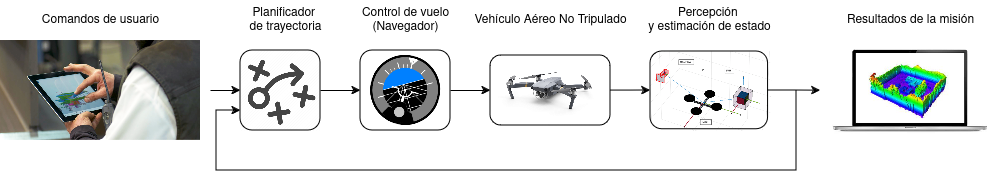
\includegraphics[width=14cm]{drone_loop}\\
\end{frame}

\begin{frame}{Perspectiva de la solución}
  \centering
  \bigskip % Vertical whitespace
  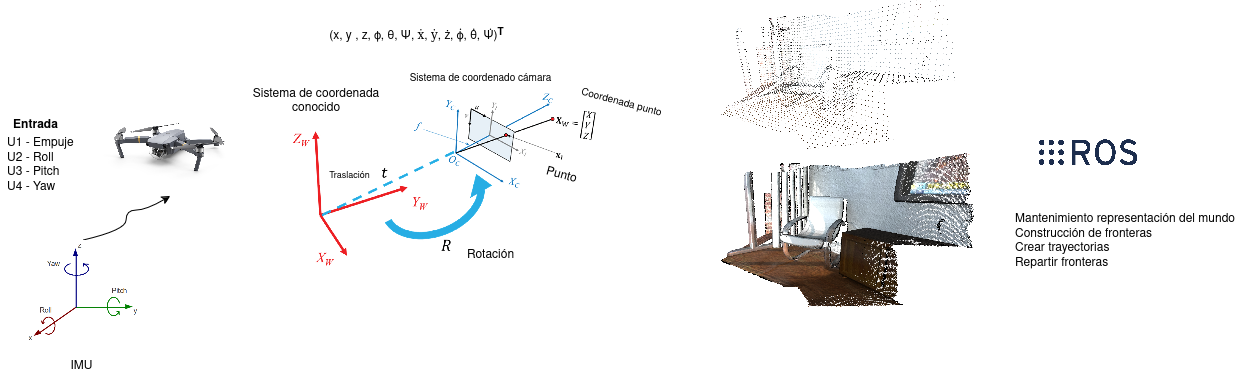
\includegraphics[width=15cm]{big_picture}\\
\end{frame}

\begin{frame}{Máquina de estados finitos}
  \centering
  \bigskip % Vertical whitespace
  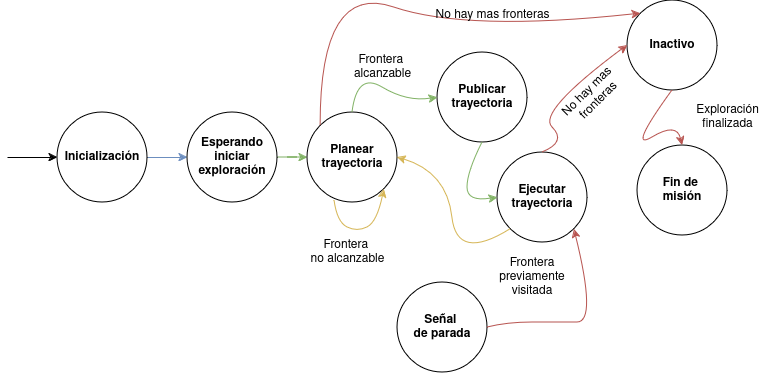
\includegraphics[width=12cm]{FSM}\\
\end{frame}

\section{Resultados a la fecha}

\begin{frame}{Simulador}
  \small
  Integración del simulador dinámico \cite{RACER2022} \footnote{\scriptsize Rapid Collaborative Exploration With a Decentralized Multi-UAV System} utilizando la odometría de referencia de los VANTS, cada agente está equipado con una cámara de profundidad que mira hacia adelante cuya resolución es 640x480px y un campo de visión de 80°x60°. Las imágenes de profundidad se generan utilizando el proceso presentado en \cite{OMNI2022} \footnote{\scriptsize Omni-Swarm: A Decentralized Omnidirectional Visual–Inertial–UWB State Estimation System for Aerial Swarms} con un rango máximo de detección de 4.5 m.
  \begin{itemize}
  \item Para usar el simulador fué necesario utilizar un contenedor docker por su portabilidad.
  \item Comprender la programación orientada a objetos C++
  \end{itemize}
\end{frame}

\begin{frame}{ROS Master}
  \begin{figure}
    \centering
    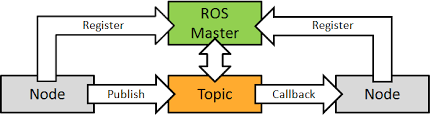
\includegraphics[width=0.5\textwidth]{ros_master}
  \end{figure}
  
  \begin{itemize}
    \item Es un servidor que provee información de conexión (dirección, notificaciones) hacia los nodos del sistema.
    \item Los mensajes son transmitidos entre los nodos vía peer-to-peer.
    \item Los nodos deben conocer la dirección del nodo maestro antes de iniciar.
    \item Los nodos son programas individuales y se organizan en paquetes.
    \item La comunicación entre nodos es mediante tópicos y es de tipo unidireccional.
  \end{itemize}
\end{frame}

\begin{frame}{Generación de un ambiente a explorar}
  \begin{figure}[ht!]
    \centering
    \begin{minipage}{0.48\textwidth}
      \centering
      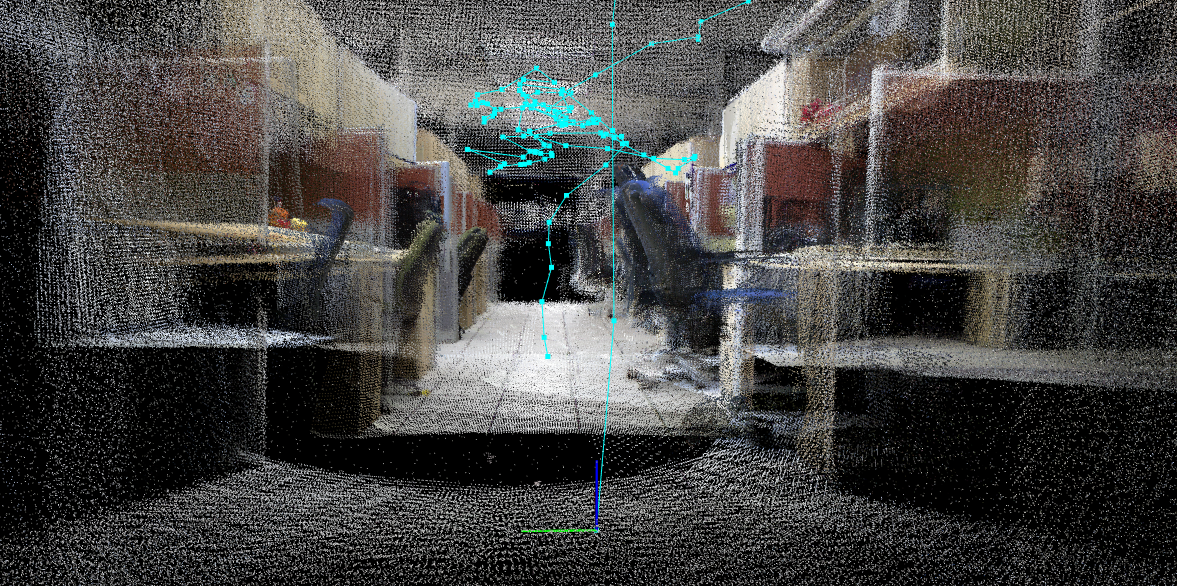
\includegraphics[width=\linewidth,height=3.5cm]{ROS_MAP2} % BUSQUEDA Y RESCATE
    \end{minipage}\hfill
    \begin{minipage}{0.48\textwidth}
      \centering
      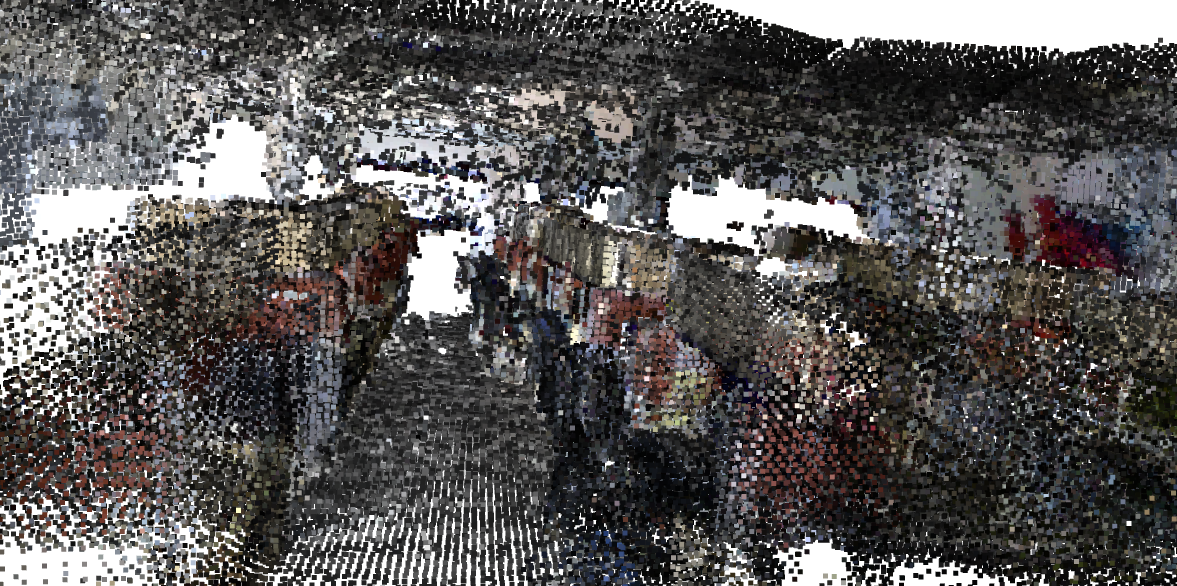
\includegraphics[width=\linewidth,height=3.5cm]{ROS_MAP3} % INSPECCION Y SEGURIDAD
    \end{minipage}
    \vspace{-0.2cm} % Espacio vertical entre imágenes
    \begin{minipage}{0.48\textwidth}
      \centering
      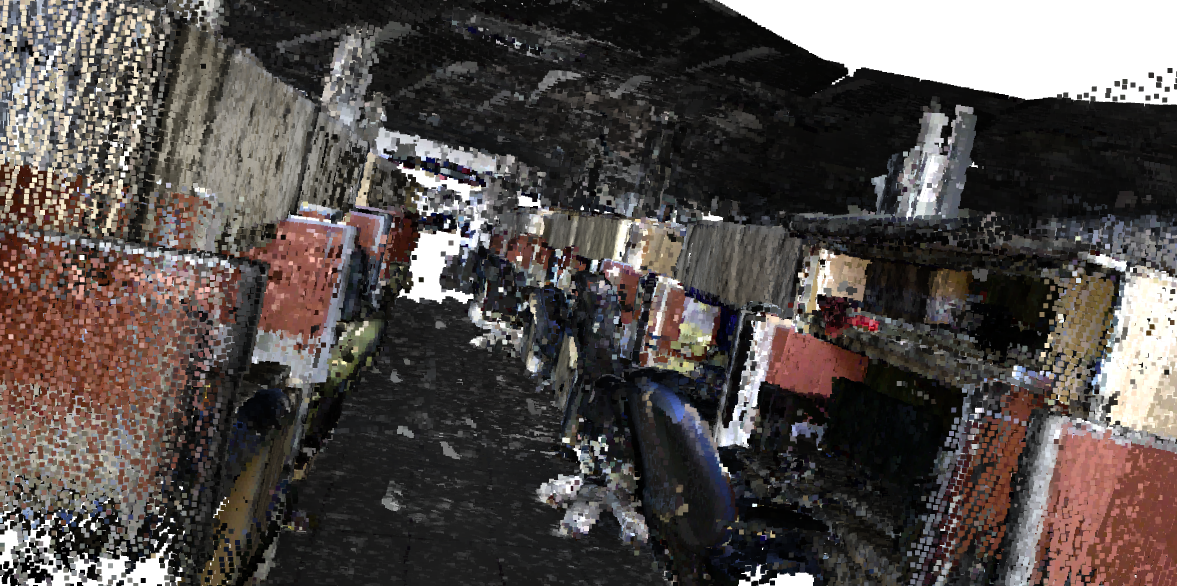
\includegraphics[width=\linewidth,height=3.5cm]{ROS_MAP4} % DRONES EN CIUDADES CON GPS DENY
    \end{minipage}\hfill
    \begin{minipage}{0.48\textwidth}
      \centering
      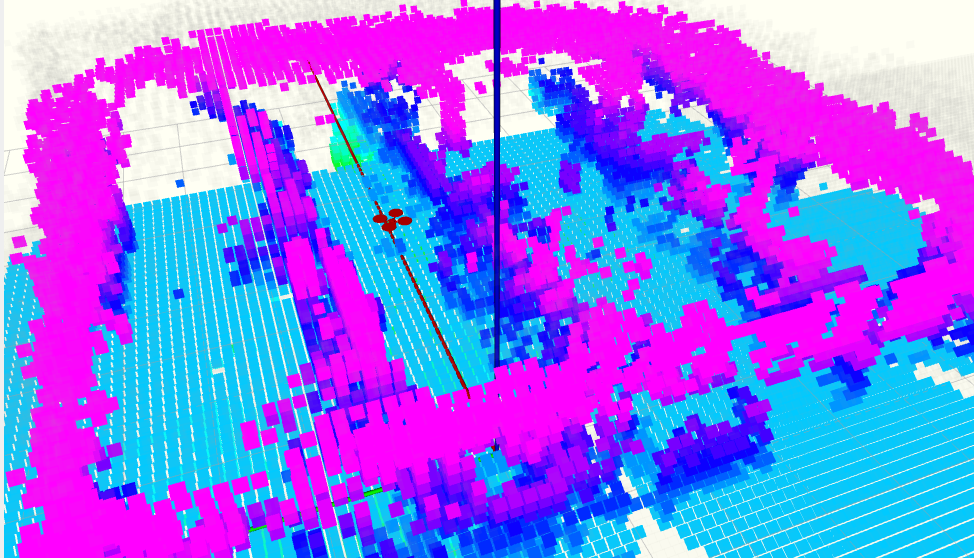
\includegraphics[width=\linewidth,height=3.5cm]{ROS_MAP6} % 
    \end{minipage}
  \end{figure}
\end{frame}

%\begin{frame}{Estructura de datos para la representación del ambiente a explorar}
%  Manejo de consultas en la estructura de datos que almacena la información de los voxels
%\end{frame}

\begin{frame}{Control de desplazamientos}
  \bigskip % Vertical whitespace
  \centering
  \animategraphics[width=0.45\textwidth,height=0.45\textheight]{10}{ros_map_1/ros_map-}{0}{300}
  \hfil
  \animategraphics[width=0.45\textwidth,height=0.45\textheight]{10}{ros_map_2/ros_map-}{0}{239}
  \vspace{2pt}\\
  \textcolor{blue}{1 VANT}
  \hfil
  \textcolor{blue}{2 VANT}
\end{frame}

\begin{frame}{Identificación de fronteras}
  \centering
  \bigskip % Vertical whitespace
  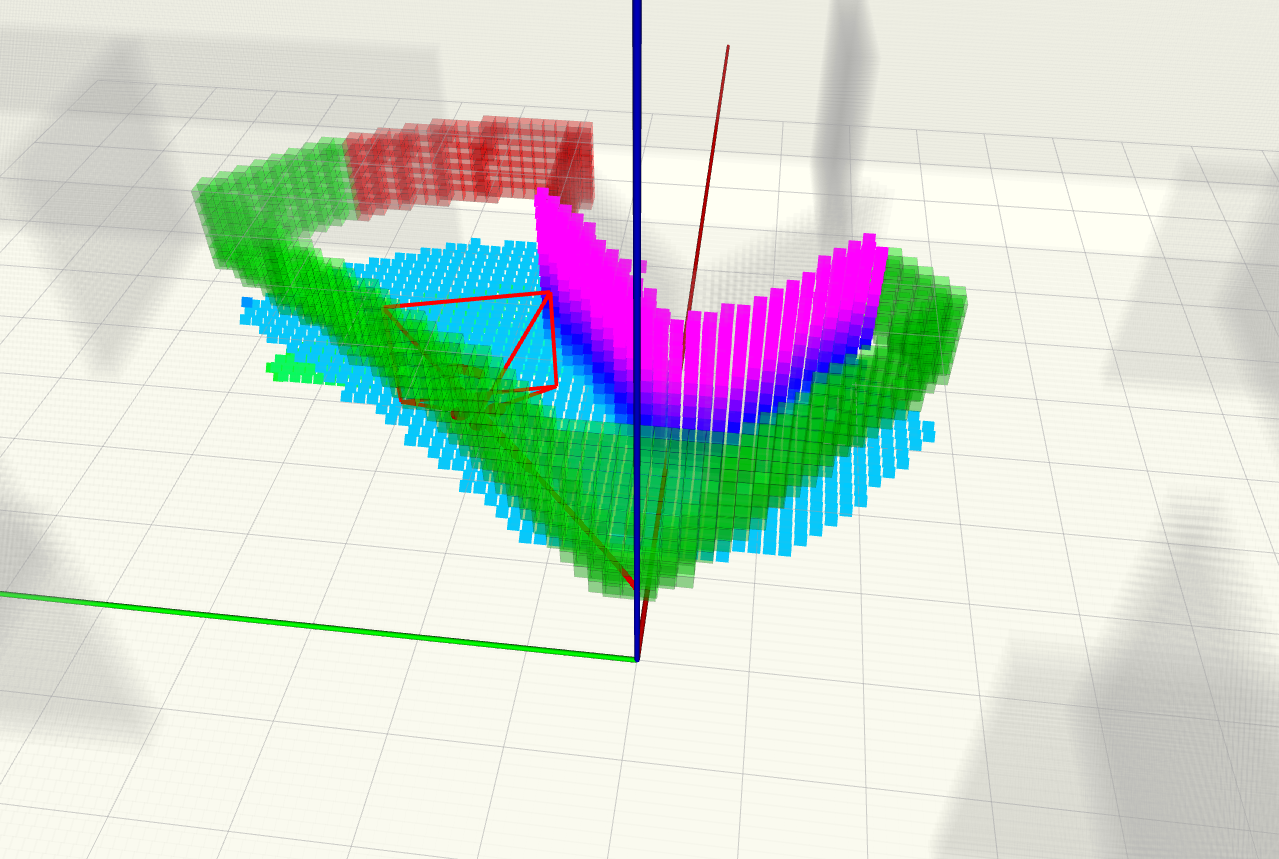
\includegraphics[width=11cm]{fronteras_ros}\\
\end{frame}
  
\begin{frame}{Grado de cumplimiento}
  
  \begin{block}{Preguntas de investigación}
    \small{
      \begin{enumerate}
      \item ¿Qué características de la dinámica del VANT son clave para generar trayectorias suaves y continuas? \\
        \progressbar[linecolor=blue, filledcolor=green]{1}\llap{\raisebox{1.5pt}{\tiny$100\%$}\hspace{0.8cm}}
      \item ¿Podría un planificador de trayectorias que aproveche las regiones libres de obstáculos acelerar los desplazamientos de los VANTs y, consecuentemente, reducir los tiempos de exploración? \\
        \progressbar[linecolor=blue, filledcolor=green]{0.5}\llap{\raisebox{1.5pt}{\tiny$50\%$}\hspace{0.8cm}}
      \item ¿Qué mecanismos de coordinación existen dentro de la literatura que podrían ayudar en resolver el problema de exploración multi-VANT? \\
        \progressbar[linecolor=blue, filledcolor=green]{1}\llap{\raisebox{1.5pt}{\tiny$100\%$}\hspace{0.8cm}}
      \end{enumerate}
    }
  \end{block}
\end{frame}

\begin{frame}{Grado de cumplimiento}
  \small
  \begin{block}{Objetivo General \progressbar[linecolor=blue, filledcolor=green]{0.57}\llap{\raisebox{1.5pt}{\tiny$57\%$}\hspace{0.8cm}}}
    \vspace{1mm}
    Desarrollar una estrategia de exploración descentralizada que permita resolver los problemas de coordinación para múltiples VANTS en ambientes desconocidos.
  \end{block}
  
  \begin{block}{Objetivos Particulares}
    %\vspace{2mm}
    \small{
      \begin{enumerate}
      \item Desarrollar una arquitectura de software que resuelva los problemas de autonomía para un VANT (localización, manejo de mapas y planificación de trayectorias).\\
        \progressbar[linecolor=blue, filledcolor=green]{1}\llap{\raisebox{1.5pt}{\tiny$100\%$}\hspace{0.8cm}}
      \item Implementar un mecanismo de coordinación descentralizado que asigne tareas de exploración. \\
        \progressbar[linecolor=blue, filledcolor=green]{0.2}\llap{\raisebox{1.5pt}{\tiny$20\%$}\hspace{0.8cm}}
      \item Realizar pruebas y simulaciones de la solución propuesta en diversos entornos, analizando la relación tiempo de exploración y cobertura del área de interés. \\
        \progressbar[linecolor=blue, filledcolor=green]{0.5}\llap{\raisebox{1.5pt}{\tiny$50\%$}\hspace{0.8cm}} 
      \end{enumerate}
    }
  \end{block}
\end{frame}

\section{Desviaciones de la investigación}
\begin{frame}
  \begin{itemize}
  \item Intentar comprender todo el panorama de VANTS en el estado del arte.
  \item Conocer los diversos métodos para la obtención de la ubicación de un VANT en un ambiente desconocido sin el uso de sensores de localización como GPS ó GNSS (Ya que se trabaja en interiores). 
  \item A pesar que la elección del simulador que se realizó en la primera etapa, su manejo y comprensión no es algo trivial.
  \item Para abordar el trabajo de exploración con múltiples VANTS se deben de resolver diversas etapas en un inicio. (Control, navegación, representación medio ambiente)
  \item Al tener dos trabajos desarrollados en el mismo simulador, es interesante tener nuestra solución implementada en el mismo y así lograr una comparativa equitativa en los resultados.
  \end{itemize}
\end{frame}

\subsection{Plan de acción para concluir la tesis}
\scriptsize
\begin{frame}{Plan de acción para concluir la tesis}
  \textcolor{red}{Prioridad Alta} Obtener los elementos que me permitan aplicar la estrategia de exploración.
  \begin{itemize}
  \item Agrupamiento de fronteras
  \item Ponderación de fonteras bajo los preceptos de exploración, explotación y cohesión
  \item Distribuir la lista de fronteras
  \end{itemize}

  Generación de canal de comunicación
  \begin{itemize}
  \item Comunicación entre agentes
  \item Cálculo de ofertas entre agentes de manera distribuida
  \end{itemize}

  \textbf{Compromiso: Julio}
  
  \textcolor{orange}{Prioridad Media} Recabar la información del desempeño de la estrategia de exploración.
  \begin{itemize}
    \item Escritura tesis
  \end{itemize}
  \textbf{Compromiso: Septiembre}
\end{frame}

%TODO
%\begin{frame}{Gantt}
%\begin{minipage}{3cm}
%\tiny{
%\begin{ganttchart}[
%hgrid style/.style={black, dotted},
%vgrid={*5{black,dotted}, *1{white, dotted}, *1{black, dashed}},
%x unit=3mm,
%y unit chart=9mm,
%y unit title=12mm,
%time slot format=isodate,
%group label font=\bfseries \Large,
%link/.style={->, thick}
%]{2024-05-06}{2024-08-23}
%\gantttitlecalendar{year, month=name, week}\\
%\ganttgroup[
%group/.append style={fill=orange}
%]{\small Etapa 2}{2024-05-06}{2024-07-26}\\ [grid]
%\ganttorangebar[
%name=VIS
%]{Visualización Datos}{2024-05-06}{2024-05-15}\\ [grid]
%\ganttorangebar[
%name=FOVSim
%]{Comprension FOV Simulador}{2024-05-15}{2024-05-20}\\ [grid]
%\ganttorangebar[
%name=Trazabilidad
%]{Trazabilidad}{2024-05-20}{2024-05-22}
%\ganttlinkedorangebar{}{2024-05-06}{2024-05-15}
%\ganttlinkedorangebar{}{2024-05-15}{2024-05-22}
%\ganttlinkedorangebar{}{2014-10-17}{2014-10-17}
%\ganttlinkedorangebar[name=FMEend]{}{2014-10-21}{2014-10-24}
%\ganttlinkedorangebar{}{2014-10-28}{2014-10-31}\\ [grid]
%\ganttorangebar[name=Manual]{Manual}{2014-10-30}{2014-10-31}
%\ganttlinkedorangebar{}{2014-11-4}{2014-11-7} \ganttnewline[thick, black]
%\ganttgroup[
%group/.append style={fill=green}
%]{KLIP Manager}{2014-11-3}{2014-11-9}
%\ganttgroup[
%group/.append style={fill=green}
%]{}{2014-11-17}{2014-11-23}\\ [grid]
%\ganttgreenbar{Manual}{2014-11-4}{2014-11-7}
%\ganttlinkedgreenbar{}{2014-11-18}{2014-11-19}
%%Implementing links
%\ganttlink[link mid=0.75]{Documentation}{FME}
%\ganttlink{FMETutorial}{FME}
%\end{ganttchart}
%}
%\end{minipage}
%\end{frame}

%\begin{frame}{Ejemplo}
%\begin{table}
%\begin{tabular}{|l|c|c|}
%foo & bar & 
%\progressbar[linecolor=blue, filledcolor=green]{0.6}\llap{\raisebox{1.5pt}{\tiny$60\%$}\hspace{0.8cm}}  \\
%foo & bar & 
%\progressbar[linecolor=blue, filledcolor=green]{0.6}%
%\begin{picture}(0,0)
%\put(-35,1.5) {\tiny$60\%$}
%\end{picture}
%\end{tabular}
%\end{table}
%\end{frame}

\begin{frame}[standout]
  ¿Preguntas?
\end{frame}

\appendix

\section{Apéndice}

%\begin{frame}[fragile]{Antecedentes}
 
  %\centering
%  Principales preguntas que un robot autónomo debe responder \footnotemark\\
%  \begin{itemize}
%  \item ¿Dónde estoy? $\implies$ Localización 
%  \item ¿A dónde voy? $\implies$ Cognición
%   \item ¿Cómo llego hasta ahí? $\implies$ Planificación de trayectoria
%   \end{itemize}
  %\pause
  %\bigskip % Vertical whitespace
%   Para resolver estas preguntas, el robot debe:\\
%   \begin{itemize}
%   \item Tener un modelo del ambiente (dado, o autónomamente construido)
%   \item Localizarse dentro del ambiente
%   \item Planear y ejecutar sus movimientos
%   \end{itemize}

%   \footnotetext{Visual map making for a mobile robot [\cite{1087348}]}
  
% \end{frame}

% \begin{frame}{Antecedentes}
%   \centering
%   \textbf{Arquitectura de un robot móvil}
%   \bigskip % Vertical whitespace
%   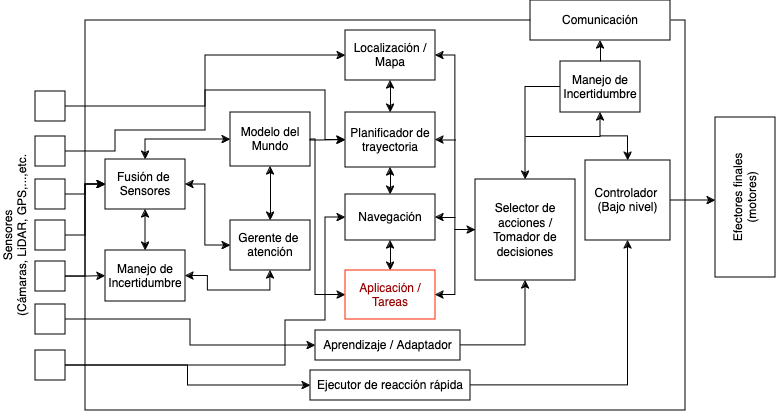
\includegraphics[width=11cm]{arquitectura_robots}\\
% \end{frame}

% \begin{frame}[fragile]{Motivación del proyecto}
  %https://ccc.inaoep.mx/~emorales/Papers/2009/eduardo.pdf
  %https://www.mdpi.com/2504-446X/7/1/62
  %Hablar de los usos e importancia del trabajo .. de la exploracion .. de la importancia de investigacion en robotica para el pais.
  %El potencial del uso de UAVs en tareas de búsqueda y rescate, inspección, mapeo, vigilancia, entre otras, es de gran interés a explorar, debido a las habilidades de vuelo que presentan en favor de la realización de estas tareas, y en especial situaciones que podrían poner en riesgo a personas.\\
  %Enviar personal de rescate dentro de un edificio parcialmente colapsado por un terremoto en busca de sobrevivientes, es poner a más personas en un gran riesgo, pues no se sabe qué es lo que les espera en el interior del edificio; esto limita la capacidad de tomar buenas decisiones acerca de si es seguro seguir cierto camino.
%   \begin{figure}[ht!]
%     \centering
%     \begin{minipage}{0.48\textwidth}
%       \centering
%       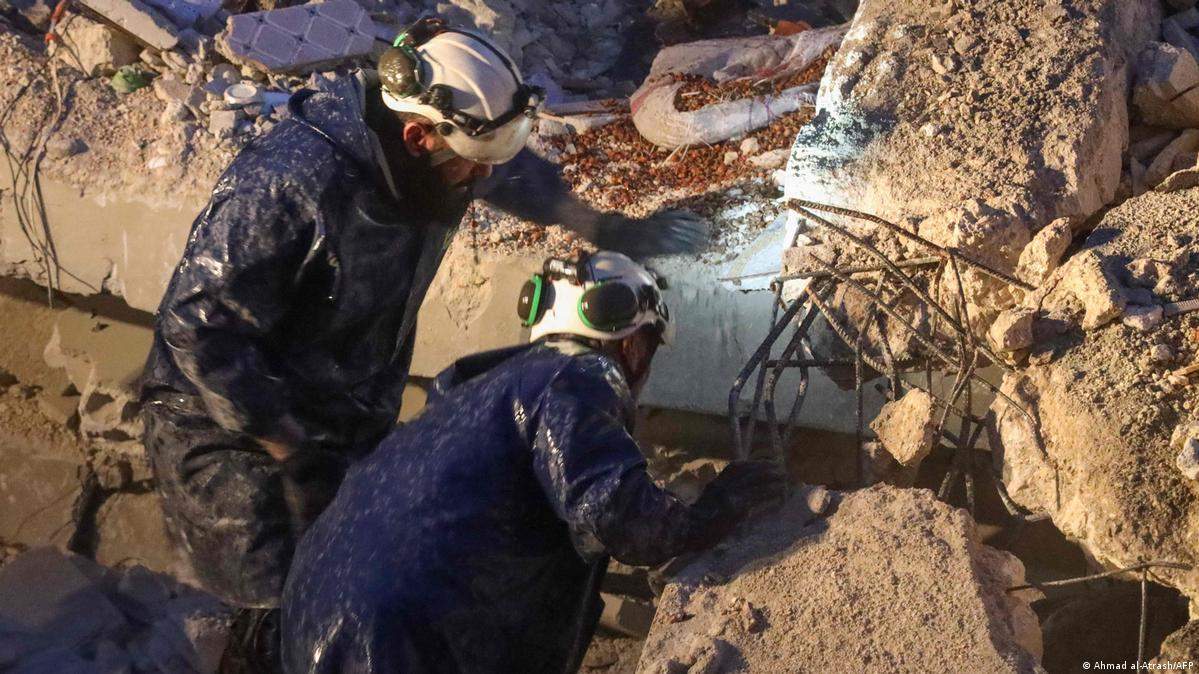
\includegraphics[width=\linewidth,height=3.5cm]{turquia1.jpg} % BUSQUEDA Y RESCATE
      %\caption{Primera Imagen}
%     \end{minipage}\hfill
%     \begin{minipage}{0.48\textwidth}
%       \centering
%       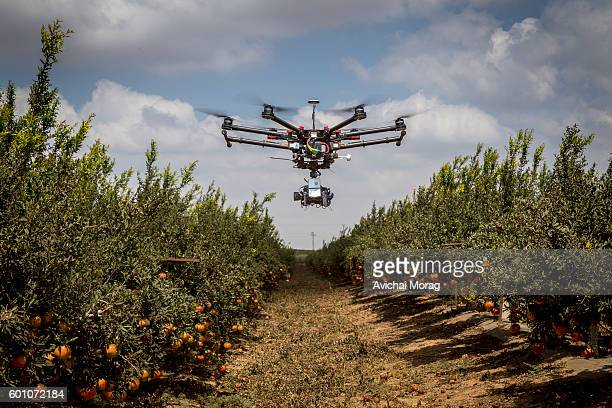
\includegraphics[width=\linewidth,height=3.5cm]{drone_agriculture.jpg} % INSPECCION Y SEGURIDAD
      %\caption{Segunda Imagen}
%     \end{minipage}
%     \vspace{-0.2cm} % Espacio vertical entre imágenes
%     \begin{minipage}{0.48\textwidth}
%       \centering
%       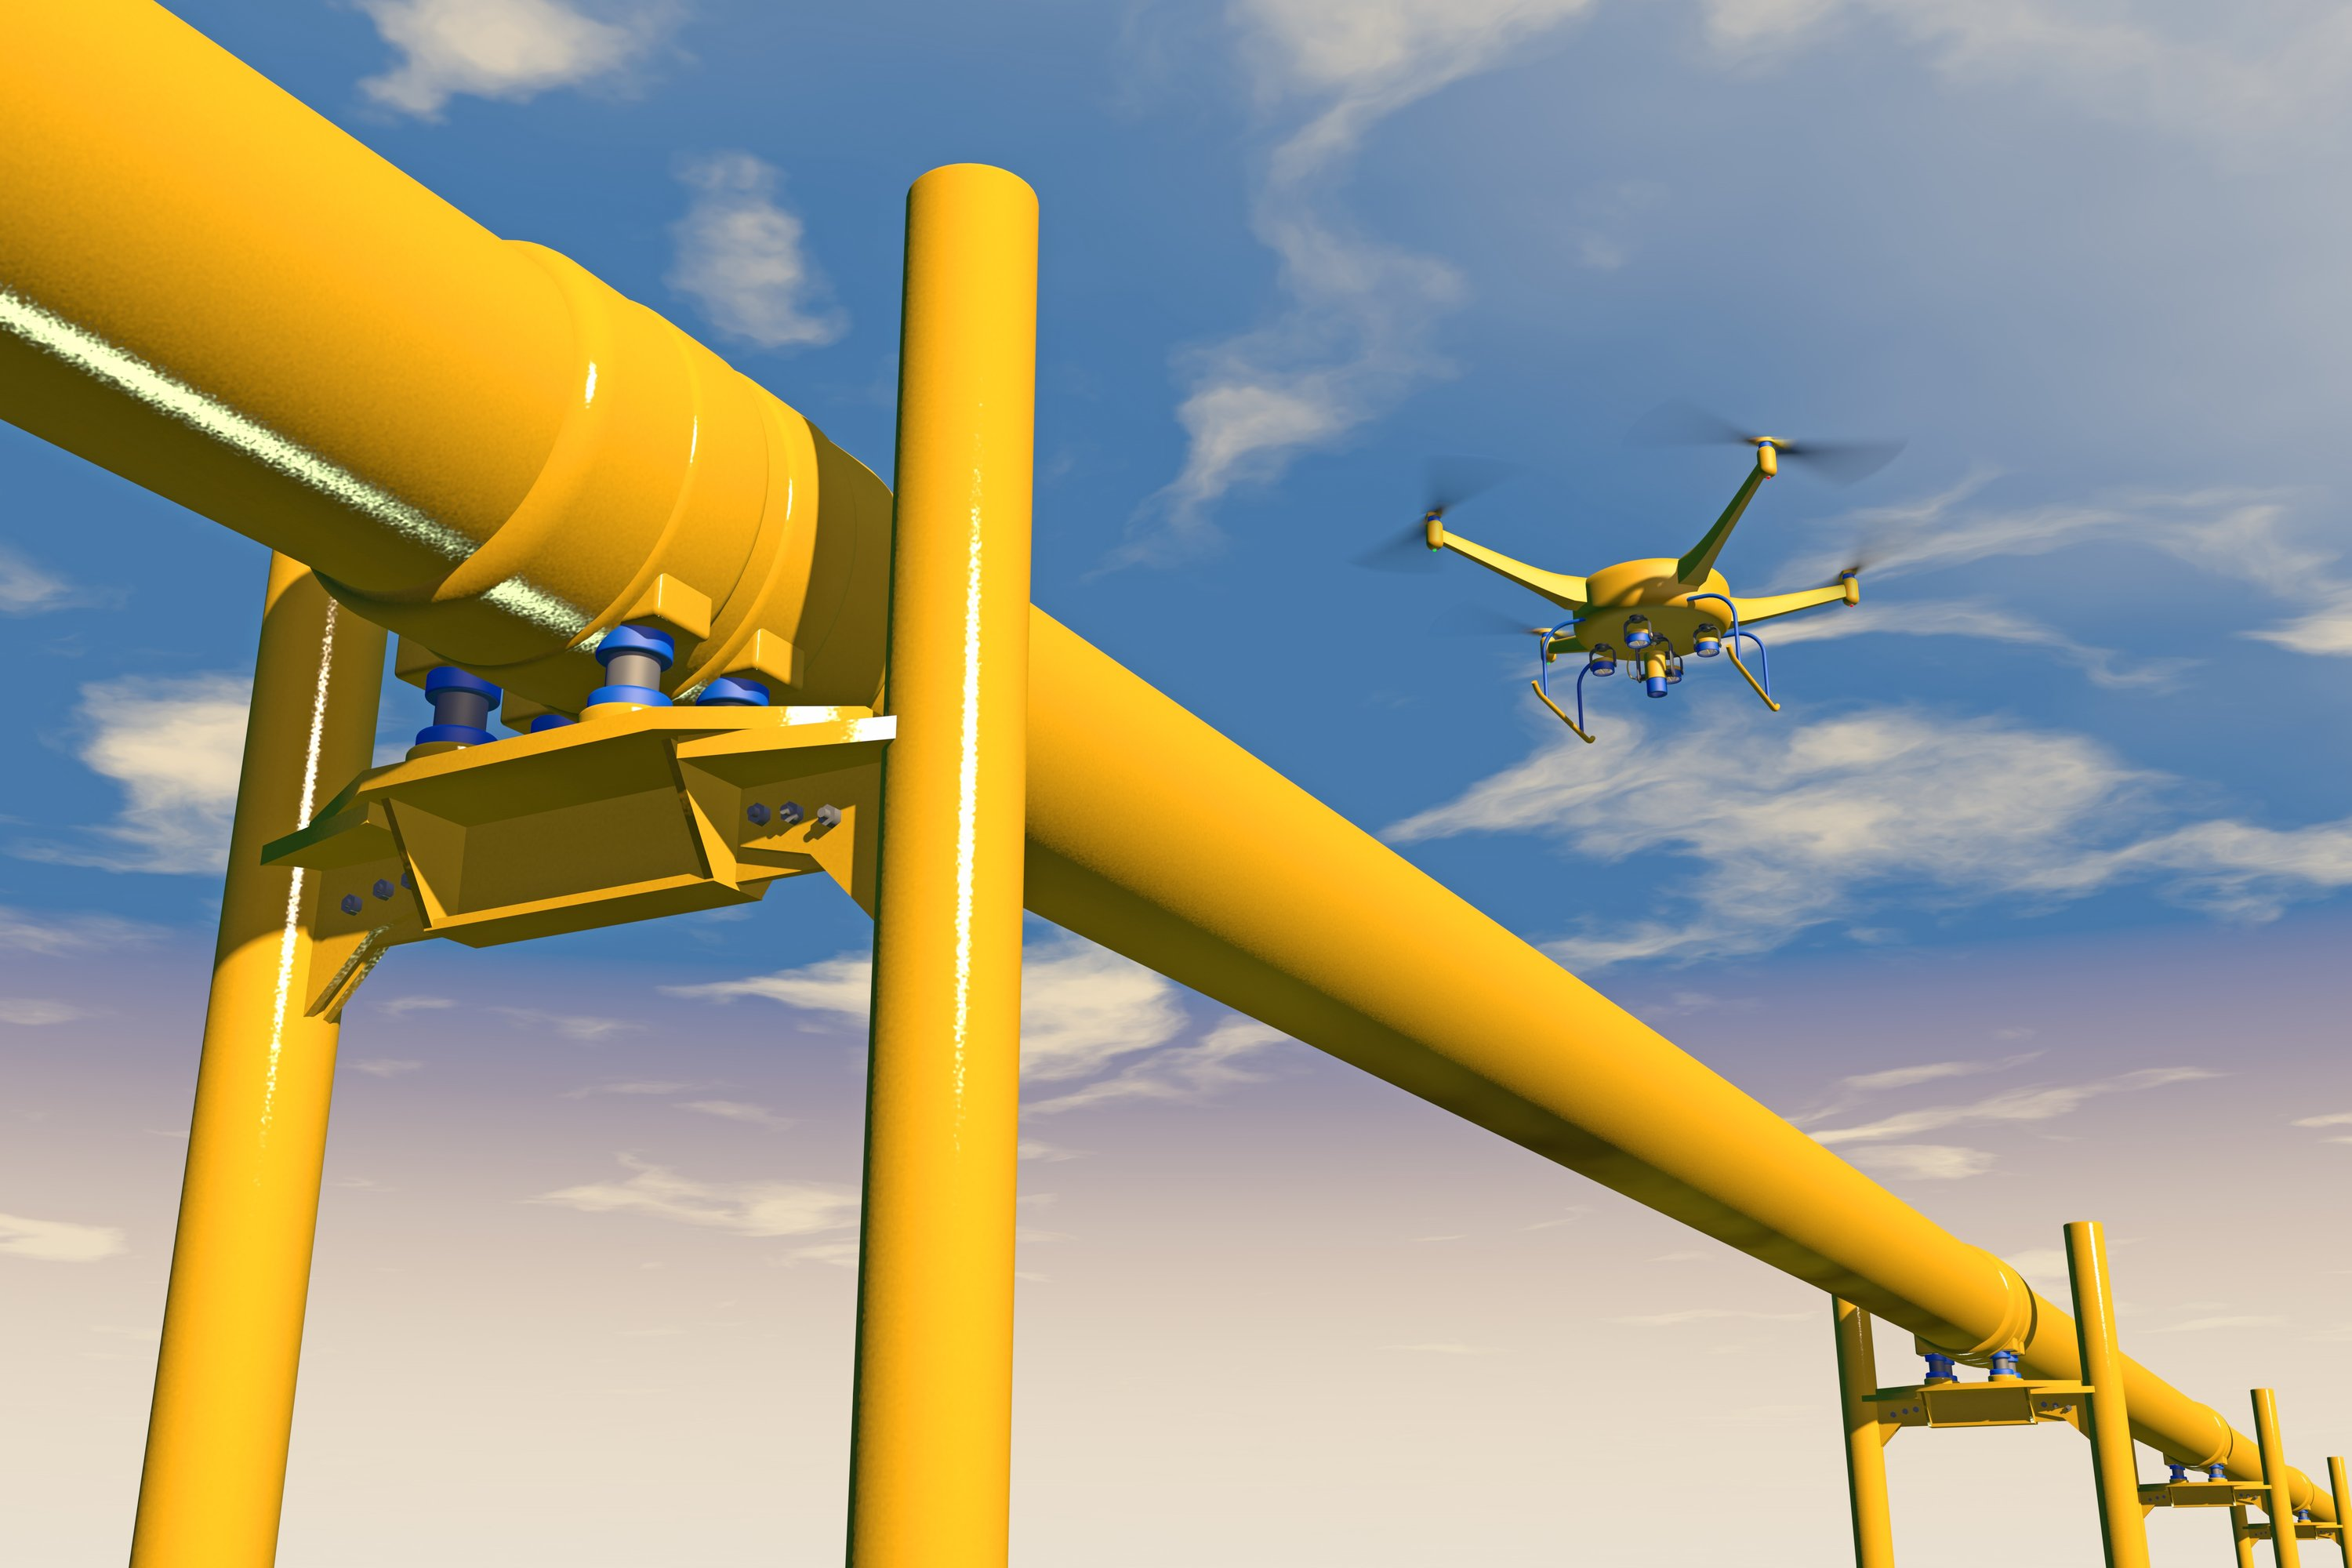
\includegraphics[width=\linewidth,height=3.5cm]{pipe_drone.jpg} % DRONES EN CIUDADES CON GPS DENY
      %\caption{Tercera Imagen}
%     \end{minipage}\hfill
%     \begin{minipage}{0.48\textwidth}
%       \centering
%       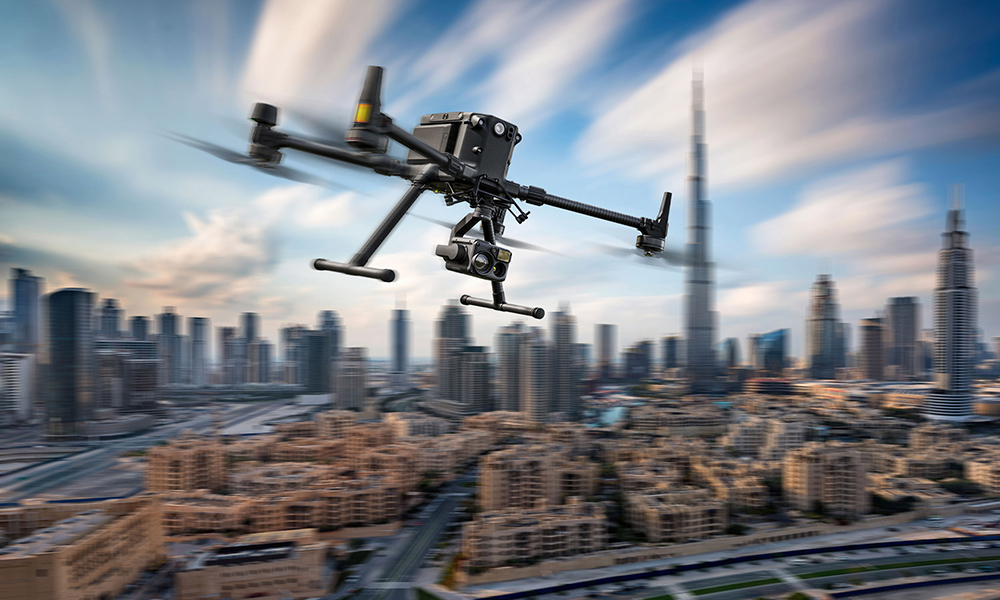
\includegraphics[width=\linewidth,height=3.5cm]{drone_city.jpg} % 
      %\caption{Cuarta Imagen}
%     \end{minipage}
%   \end{figure}
% \end{frame}


% \begin{frame}{Robot autónomo}
%   \centering
%   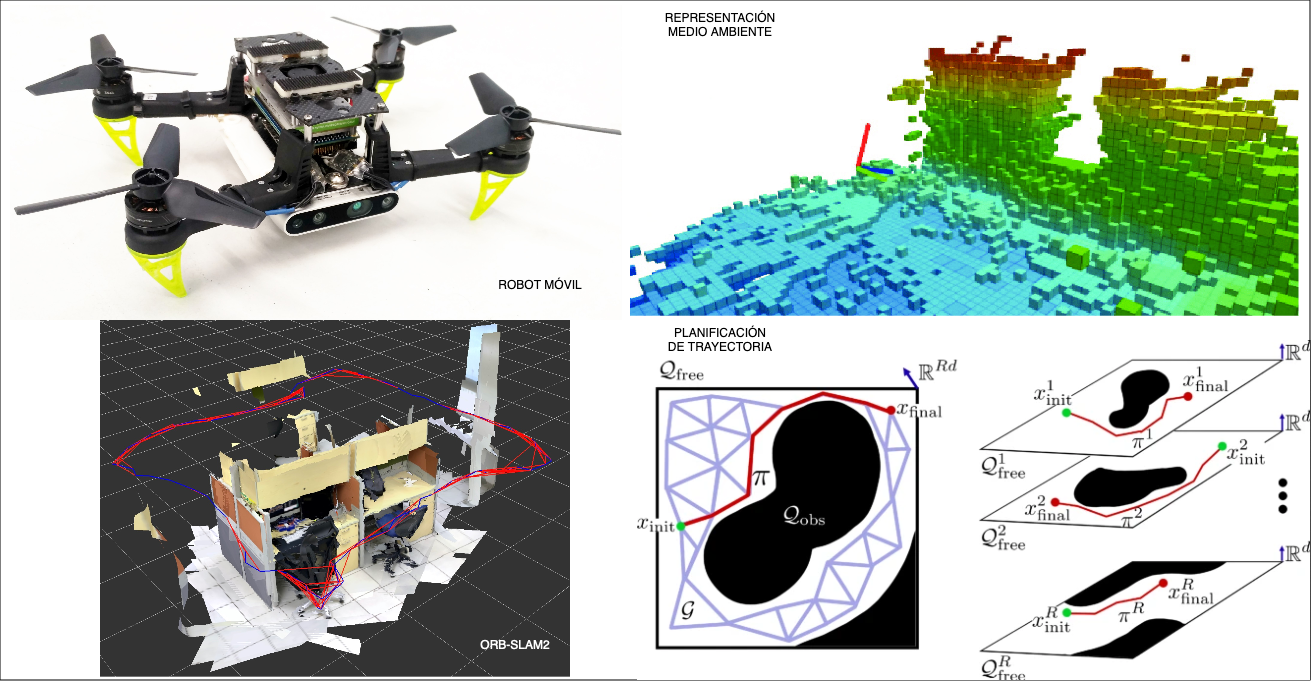
\includegraphics[width=\linewidth]{ANTECEDENTES}\\
% \end{frame}

% \begin{frame}{Control de un VANT \footnote{Modeling And Control Of A Quadrotor Uav With Aerodynamic Concepts, [\cite{1334249}]}}
  
%   \begin{minipage}{0.47\textwidth}
     
%     Estados del VANT \\
%     $(x,y,z,\phi,\theta,\Psi,\dot{x},\dot{y},\dot{z},\dot{\phi},\dot{\theta},\dot{\Psi})^\mathrm{T}$

%     \bigskip % Vertical whitespace
    
%     Donde:
%     \begin{itemize}
%     \item $\xi = (x,y,z)^\mathrm{T}$ representan la posición linear
%     \item $\eta = (\phi,\theta,\Psi)^\mathrm{T}$ ángulos de euler: roll, pitch, yaw
%     \item $(\dot{x},\dot{y},\dot{z},\dot{\phi},\dot{\theta},\dot{\Psi})^\mathrm{T}$ velocidades lineares y angulares
%     \end{itemize}
%   \end{minipage}
%   \hspace{0.2cm}
%   \begin{minipage}{0.5\textwidth}
%     \centering
%     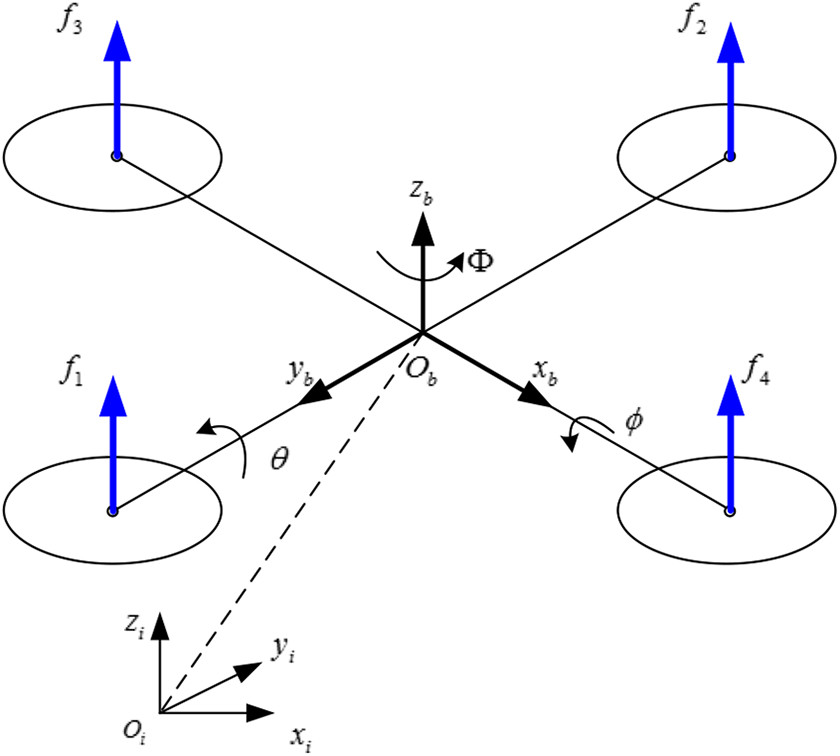
\includegraphics[width=4cm]{uav_model.jpeg}
%     \bigskip % Vertical whitespace
%     {\scriptsize
%       \begin{itemize}
%       \item Cuatro rotores.
%       \item Seis grados de libertad (3 lineales y 3 angulares).
%       \item Requiere cuatro variables de control $(u_1, u_2, u_3, u_4)$ para mantener su estabilidad y control durante el vuelo.
%       \end{itemize}
%     }
%   \end{minipage}
%   \bigskip % Vertical whitespace
% \end{frame}

% \begin{frame}{Formulación del Problema de Localización y Mapeo Simultáneos \footnote{\tiny Omni-Swarm: A Decentralized Omnidirectional Visual–Inertial–UWB State Estimation System for Aerial Swarms, [\cite{OMNI2022}]}}

%   \small{
%     Dados:
%     \begin{itemize}
%     \item Conjunto de observaciones $z(t) = \{z_1,z_2,...,z_t\}$
%     \item Conjunto de comandos de control $u(t) = \{u_1,u_2,...,u_t\}$
%     \end{itemize}
    %\bigskip % Vertical whitespace
%     Requerimos:
%     \begin{itemize}
%     \item Mapa del ambiente $m$
%     \item Trayectoria del robot $x(t) = \{x_1,x_2,...,x_t\}$
%     \end{itemize}
    %\bigskip % Vertical whitespace
    
%     En terminos probabilisticos, queremos estimar la trayectoria del robot y el mapa
%   }
%   \centering
%   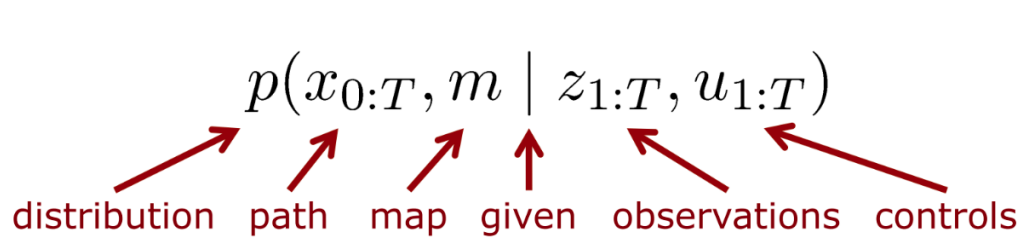
\includegraphics[width=8cm]{slam1}
%   \bigskip % Vertical whitespace
% \end{frame}

% \begin{frame}{Formulación del Problema de Localización y Mapeo Simultáneos \footnote{\tiny Omni-Swarm: A Decentralized Omnidirectional Visual–Inertial–UWB State Estimation System for Aerial Swarms, [\cite{OMNI2022}]}}
  
%   \begin{itemize}
%   \item La trayectoria del robot y el mapa son desconocidos.
%   \item Correlación entre el mapa y las posiciones del robot.
%   \end{itemize}
  
%   \centering
%   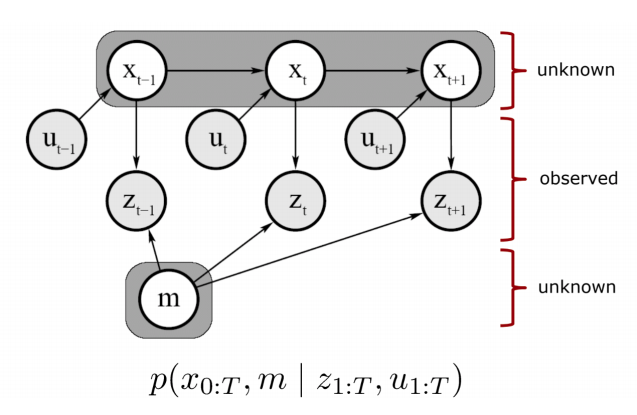
\includegraphics[width=8cm]{slam2}
%   \bigskip % Vertical whitespace
% \end{frame}

% \begin{frame}{Representación medio ambiente \footnote{\tiny RACER: Rapid Collaborative Exploration With a Decentralized Multi-UAV System [\cite{RACER2022}]}}
%   \begin{figure}[ht!]
%     \centering
%     \begin{minipage}{0.48\textwidth}
%       \centering
%       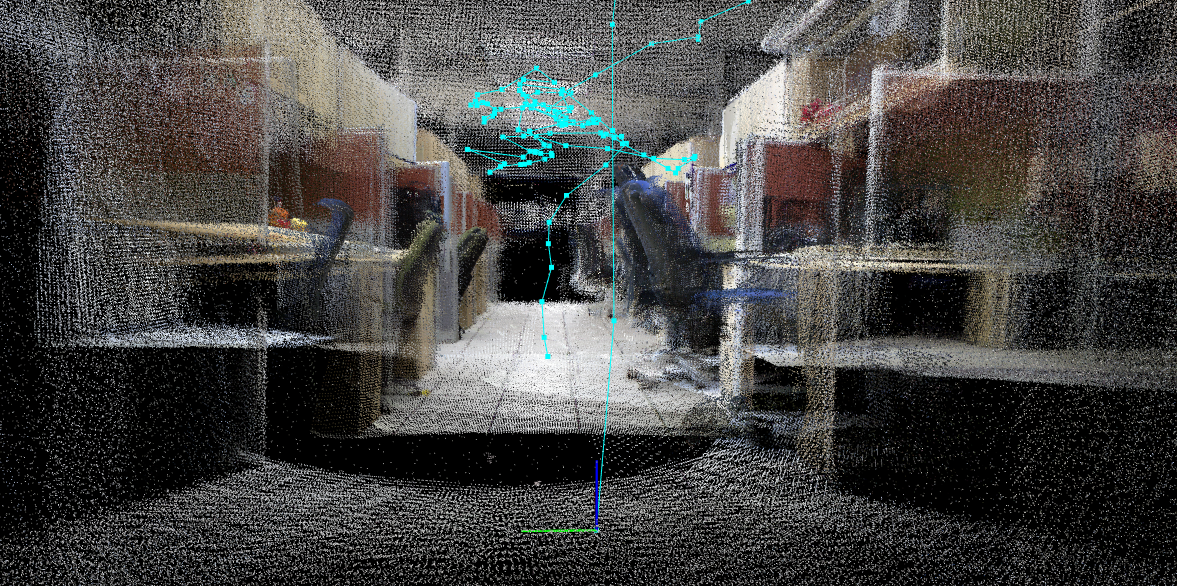
\includegraphics[width=\linewidth,height=3.5cm]{ROS_MAP2} % BUSQUEDA Y RESCATE
%     \end{minipage}\hfill
%     \begin{minipage}{0.48\textwidth}
%       \centering
%       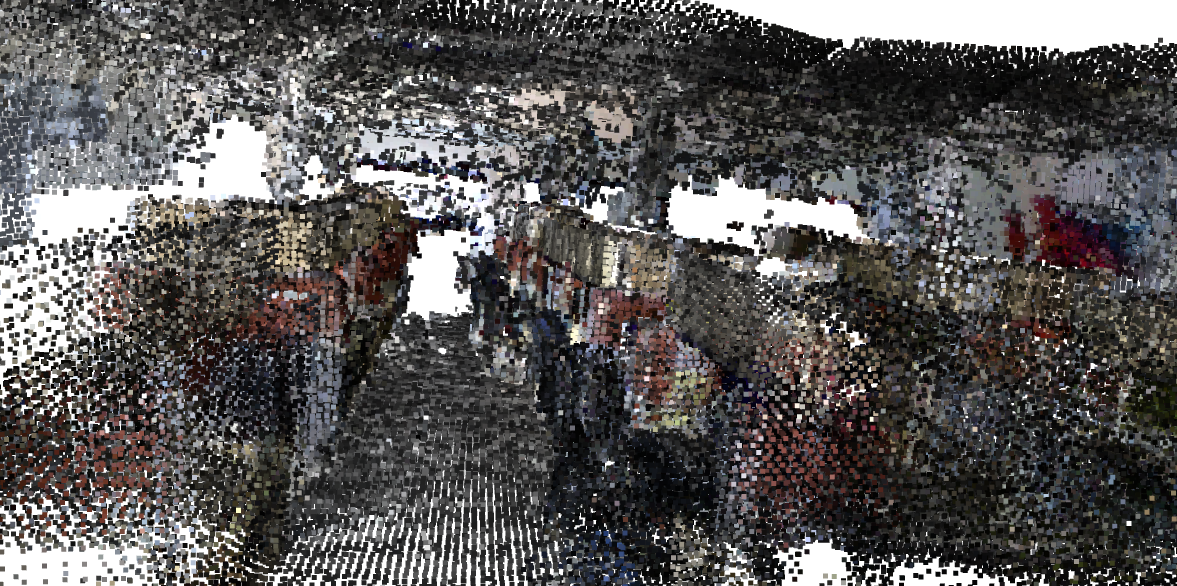
\includegraphics[width=\linewidth,height=3.5cm]{ROS_MAP3} % INSPECCION Y SEGURIDAD
%     \end{minipage}
%     \vspace{-0.2cm} % Espacio vertical entre imágenes
%     \begin{minipage}{0.48\textwidth}
%       \centering
%       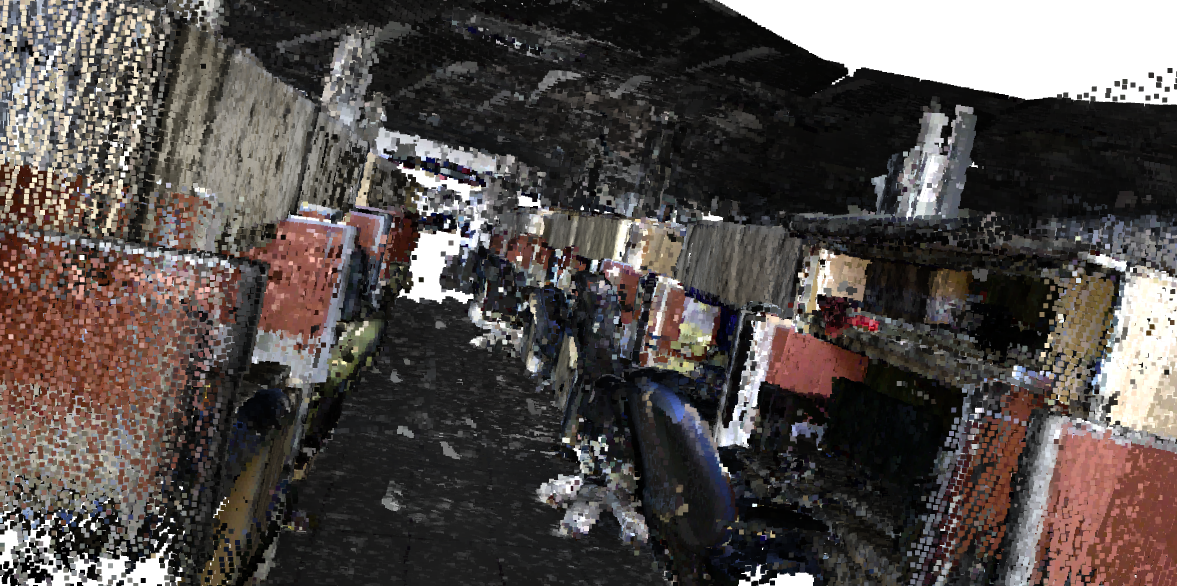
\includegraphics[width=\linewidth,height=3.5cm]{ROS_MAP4} % DRONES EN CIUDADES CON GPS DENY
%     \end{minipage}\hfill
%     \begin{minipage}{0.48\textwidth}
%       \centering
%       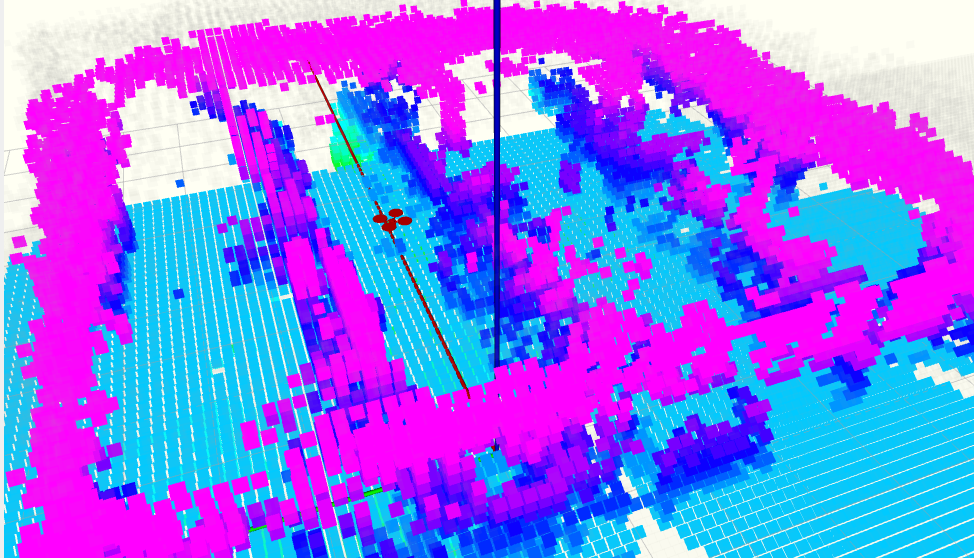
\includegraphics[width=\linewidth,height=3.5cm]{ROS_MAP6} % 
%     \end{minipage}
%   \end{figure}
%   \bigskip % Vertical whitespace
% \end{frame}

\section*{Plan de cierre del trabajo}

\begin{frame}{Cronograma inicial}
  \bigskip % Vertical whitespace
  \tiny
  %\hspace{0.0cm}
  \begin{minipage}{5cm}
    \noindent\begin{tabular}{|p{0.9\textwidth}*{16}{|p{0.029\textwidth}}|}
    % The top line
    %\diagbox[width=12.5em]{Actividades}{Cuatrimestres}
    \hline
    & \multicolumn{4}{c|}{\color{teal!80}\textbf{Cuatrimestre 4}} 
    & \multicolumn{4}{c|}{\color{teal!80}\textbf{Cuatrimestre 5}} 
    & \multicolumn{4}{c|}{\color{teal!80}\textbf{Cuatrimestre 6}}
    & \multicolumn{4}{c|}{\textbf{Cuatrimestre Extra}}\\
    \hline
    % The second line, with its five years of four quarters
    %\textcolor{black}{\textbf{Etapas}}
    \rpt[4]{& 1 & 2 & 3 & 4} \\
    \hline
    \rowcolor{teal!40}{\textbf{Etapa 1}}\\
    % using the on macro to fill in twenty cells as `on'
    %\specialcell{Actividad 1\\espacio}        \on[0] \off[12] \\
    %Actividad 1    \on[0] \off[12]\\
    \hline
    \rowcolor{teal!15}{\textbf{E1.A1.} Revisi\'{o}n literatura relevante}
    %en exploraci\'{o}n multi-VANT, estrategias de exploraci\'{o}n, algoritmos de coordinaci\'{o}n y evaci\'{o}n de obst\'{a}culos
    \onok[9] \on[7]\\
    \hline
    %\textbf{E1.A2.} Evaluaci\'{o}n de aptitudes\footnote{Evaluaci\'{o}n a partir de los nuevos trabajos}     \on[12] \\
    %\hline
    \rowcolor{teal!15}{\textbf{E1.A2.} Selecci\'{o}n de algoritmos} \onok[2] \off[14] \\
    \hline
    \rowcolor{teal!15}{\textbf{E1.A3.} Dise\~{n}o de la arquitectura de software}
    \off[1] \onok[3] \on[0] \off[12] \\
    \hline
    \rowcolor{teal!15}{\textbf{E1.A4.} Documentaci\'{o}n Etapa 1}
    \onok[4] \on[0]  \off[12] \\
    \hline
    \rowcolor{teal!15}{\textbf{E1.A5.} Revisi\'{o}n de tesis Etapa 1}
    \off[3] \onok[1]  \off[12] \\
    \hline
    % using the on macro followed by the off macro
    \rowcolor{teal!40}{\textbf{Etapa 2}}\\
    \hline
    \rowcolor{teal!15}{\textbf{E2.A1.} Selecci\'{o}n Simulador}
    \onok[1]  \off[15] \\
    \hline
    \rowcolor{teal!15}{\textbf{E2.A2.} Visualizaci\'{o}n de datos}
    \off[1] \onok[2] \ondelay[6]  \off[7] \\
    \hline
    \rowcolor{teal!7}\textbf{E2.A3.} Control de desplazamientos
    \off[2] \onok[2] \ondelay[6] \off[6] \\
    \hline
    \rowcolor{teal!7}\textbf{E2.A4.} Desarrollo de algoritmo de exploración
    \off[3] \onok[2] \ondelay[5] \off[6] \\
    \hline
    %\rowcolor{teal!15}{\textbf{E2.A5.} Implementaci\'{o}n y simulaci\'{o}n}
    %\off[3] \onok[2] \ondelay[2] \off[5] \\
    %\hline
    %\textbf{E2.A6.} Simulaci\'{o}n un solo VANT
    %\off[4] \on[1] \off[7] \\
    %\hline
    \rowcolor{teal!7}\textbf{E2.A5.} Desarrollo de algoritmo de coordinaci\'{o}n
    \off[4] \on[3] \ondelay[4] \off[5] \\
    \hline
    \rowcolor{teal!7}{\textbf{E2.A6.} Implementaci\'{o}n y simulaci\'{o}n}
    \off[3] \onok[5] \ondelay[3] \off[5] \\
    \hline
    %\textbf{E2.A9.} Simulaci\'{o}n multi-VANT
    %\off[6] \on[1] \off[5] \\
    %\hline
    \rowcolor{teal!15}{\textbf{E2.A7.} Documentaci\'{o}n Etapa 2}
    \off[4] \onok[4] \off[8] \\
    \hline
    \rowcolor{teal!15}{\textbf{E2.A8.} Revisi\'{o}n de tesis Etapa 2}
    \off[7] \onok[1] \off[8] \\
    \hline
    \rowcolor{black!5}{\textbf{Etapa 3}}\\
    \hline
    \textbf{E3.A1.} Experimentaci\'{o}n de soluci\'{o}n
    \off[10]  \on[2] \off[4] \\
    \hline
    \textbf{E3.A2.} Recopilaci\'{o}n resultados
    \off[11]  \on[1] \off[4] \\
    \hline
    \textbf{E3.A3.} Documentaci\'{o}n Etapa 3
    \off[9] \on[3] \off[4] \\
    \hline
    \textbf{E3.A4.} Revisi\'{o}n de tesis
    \off[11] \on[3] \off[2]\\
    \hline
    \textbf{E3.A5.} Divulgaci\'{o}n
    \off[12]  \on[3] \off[1]\\
    \hline
    \textbf{E3.A6.} Proceso de titulaci\'{o}n
    \off[14] \on \off[1]\\
    \hline
    \end{tabular}
  \end{minipage}
\end{frame}

\begin{frame}
  \bigskip % Vertical whitespace
  \tiny
  \scalebox{0.75}{  
  %\hspace{0.0cm}
    \begin{minipage}{1cm}
    \noindent\begin{tabular}{|p{11.5\textwidth}*{16}{|p{0.002\textwidth}}|}
    % The top line
    %\diagbox[width=12.5em]{Actividades}{Cuatrimestres}
    \hline
    & \multicolumn{4}{c|}{\color{teal!80}\textbf{MAYO}} 
    & \multicolumn{4}{c|}{\textbf{JUNIO}} 
    & \multicolumn{4}{c|}{\textbf{JULIO}}
    & \multicolumn{4}{c|}{\textbf{AGOSTO}}\\
    \hline
    % The second line, with its five years of four quarters
    %\textcolor{black}{\textbf{Etapas}}
    \rpt[4]{& 1 & 2 & 3 & 4} \\
    \hline
    \rowcolor{teal!40}{\textbf{Visualización de datos}}\\
    \hline
    \rowcolor{teal!15}\textbf{A1.} Manejo estructura del mapa
    \onok[2] \off[14] \\
    \hline
    \rowcolor{teal!15}\textbf{A2.} Comprensión del FOV aplicado dentro del simulador
    \off[1] \onok[2] \off[13] \\
    \hline
    \rowcolor{teal!15}\textbf{A3.} Trazabilidad de la trayectoria
    \off[2] \onok[2] \off[12] \\
    \hline
    \rowcolor{teal!15}\textbf{A4.} Manejo de los mensajes en ROS
    \off[2] \onok[2] \off[12] \\
    \hline
    \rowcolor{teal!15}{\textbf{A5.} Manejo de los tópicos en ROS}
    \off[2] \onok[2] \off[12] \\
    \hline
    \rowcolor{teal!40}{\textbf{Control de desplazamientos}}\\
    \hline
    \textbf{A1.} Comprención de la ejecución del algoritmo A* en $\mathbb{R}^{3}$
    \off[4]  \on[1] \off[11] \\
    \hline
    \textbf{A2.} Aplicación de planificador local PVA
    \off[4]  \on[2] \off[10] \\
    \hline
    \rowcolor{teal!40}{\textbf{Desarrollo de algoritmo de exploración}}\\
    \hline
    \textbf{A1.} Manejo de pase de mapas entre agentes
    \off[5]  \on[2] \off[9] \\
    \hline
    \textbf{A2.} Clusterización de regiones de fronteras
    \off[4]  \on[2] \off[10] \\
    \hline
    \textbf{A3.} Integración de los mapas de los agentes
    \off[6]  \on[2] \off[8] \\
    \hline
    \rowcolor{teal!40}{\textbf{Desarrollo de coordinación}}\\
    \hline
    \textbf{A1.} Solución greedy
    \off[8]  \on[1] \off[7] \\
    \hline
    \textbf{A2.} Solución branch \& bound
    \off[9]  \on[1] \off[6] \\
    \hline
    \textbf{A3.} Solución método húngaro
    \off[10]  \on[1] \off[5] \\
    \hline
    \rowcolor{teal!40}{\textbf{Implementación y simulación}}\\
    \hline
    \textbf{A1.} Coordinación del funcionamiento de los componentes de la arquitectura de software
    \off[8]  \on[3] \off[5] \\
    \hline
    \rowcolor{teal!40}{\textbf{Experimentación de resultados}}\\
    \hline
    \textbf{A1.} Ejecuciones entre las soluciones del estado del arte que su implementación se haya realizado en un ambiente en ROS
    \off[11]  \on[1] \off[4] \\
    \hline
    \textbf{A2.} Ejecuciones con números diferentes de VANTS
    \off[11]  \on[1] \off[4] \\
    \hline
    \rowcolor{teal!40}{\textbf{Recopilación de resultados}}\\
    \hline
    \textbf{A1.} Comparación resultados con estado del arte y con los tiempos en los diferentes mecanismos de coordinación
    \off[11]  \on[2] \off[3] \\
    \hline
    \rowcolor{teal!40}{\textbf{Documentación etapa 3}}\\
    \hline
    \textbf{A1.} Escribir cápitulos de la tesis
    \off[5]  \on[3] \off[2] \on[6]\\
    \hline
    \textbf{A2.} Redactar manuscrito CCE 2024 - IEEE
    \off[5]  \on[5] \off[6] \\
    \hline
    \textbf{A3.} Modificar correcciones
    \off[8]  \on[2] \off[1] \on[5]\\
    \hline
    \rowcolor{teal!40}{\textbf{Revisión de tesis}}\\
    \hline
    \textbf{A1.} Correcciones de revisión 1
    \off[12]  \on[4] \\
    \hline
    \textbf{A2.} Correcciones de revisión 2
    \off[12]  \on[4] \\
    \hline
    \textbf{A3.} Correcciones de revisión 3
    \off[12]  \on[4] \\
    \hline
    \end{tabular}
  \end{minipage}
  }
\end{frame}

\begin{frame}{}
  \bigskip % Vertical whitespace
  \tiny
  \scalebox{0.64}{
    \begin{minipage}{1cm}
      \begin{table}[h!]
        \begin{tabular}{|m{7cm}|m{5cm}|m{9cm}|}
          \hline
          \rowcolor{teal!40}\multicolumn{3}{|l|}{\textbf{Visualización de datos}}\\\hline
          \rowcolor{teal!15}\textbf{Actividad} & \textbf{Producto} & \textbf{Incidencia}\\\hline
          \textbf{A1} Manejo estructura del mapa & Consultas a la estructura del mapa & \multirow{5}{*}{Inversión extra de tiempo para el estudio de C++, impactando en el desarrollo del proyecto} \\
          \cline{1-2}
          \textbf{A2} Comprensión del FOV aplicado dentro del simulador & N/A &\\
          \cline{1-2}
          \textbf{A3} Trazabilidad de la trayectoria & Manejo de arreglo de las trayectorias & \\
          \cline{1-2}
          \textbf{A4} Manejo de los mensajes en ROS & Paso de argumentos al launchfile & \\
          \cline{1-2}
          \textbf{A5} Manejo de los tópicos en ROS & Manejo de tópicos dentro del nodo de ROS & \\
          \hline
          \rowcolor{teal!40}\multicolumn{3}{|l|}{\textbf{Control de desplazamientos}}\\\hline
          \rowcolor{teal!15}\textbf{Actividad} & \textbf{Producto} & \textbf{Incidencia} \\
          \hline
          \textbf{A1} Comprención de la ejecución del algoritmo A* en $\mathbb{R}^{3}$ & N/A & \multirow{2}{*}{Desempeño insuficiente para el planificador local}\\
          \cline{1-2}
          \textbf{A2} Desarrollo de planificador local PVA & Programa del planificador local & \\
          \hline
          \rowcolor{teal!40}\multicolumn{3}{|l|}{\textbf{Desarrollo de algoritmo de exploración}}\\\hline
          \rowcolor{teal!15}\textbf{Actividad} & \textbf{Producto} & \textbf{Incidencia} \\
          \hline
          \textbf{A1} Manejo de pase de mapas entre agentes & N/A & \multirow{3}{*}{Desempeño insuficiente en la homologación de los mapas}\\
          \cline{1-2}
          \textbf{A2} Clusterización de regiones de fronteras & Programa para identificar las velocidades admisibles & \\
          \cline{1-2}
          \textbf{A3} Integración de los mapas de los agentes & Construcción del mapa de la misión & \\
          \hline
          \rowcolor{teal!40}\multicolumn{3}{|l|}{\textbf{Desarrollo de algoritmo de coordinación}}\\\hline
          \rowcolor{teal!15}\textbf{Actividad} & \textbf{Producto} & \textbf{Incidencia} \\
          \hline
          \textbf{A1} Solución greedy & Programa con solución greedy & \multirow{3}{*}{Problemas en la implementación en el lenguaje C++}\\
          \cline{1-2}
          \textbf{A2} Solución branch \& bound & Programa con solución branch \& bound & \\
          \cline{1-2}
          \textbf{A3} Solución método húngaro  & Programa con solución método húngaro & \\
          \hline
          \rowcolor{teal!40}\multicolumn{3}{|l|}{\textbf{Implementación y simulación}}\\\hline
          \rowcolor{teal!15}\textbf{Actividad} & \textbf{Producto} & \textbf{Incidencia} \\
          \hline
          \textbf{A1} Coordinación del funcionamiento de los componentes de la arquitectura de software & Archivo lauchfile variando el tipo de coordinación & Problemas en la implementación en el lenguaje C++\\
          \hline
          \rowcolor{teal!40}\multicolumn{3}{|l|}{\textbf{Experimentación de resultados}}\\\hline
          \rowcolor{teal!15}\textbf{Actividad} & \textbf{Producto} & \textbf{Incidencia} \\
          \hline
          \textbf{A1} Ejecuciones entre las soluciones del estado del arte que su implementación se haya realizado en un ambiente en ROS & Gráficos de tiempos de ejecución & \multirow{2}{*}{No poder replicar los resultados en el equipo adecuado o sugeridos en el estado del arte}\\
          \cline{1-2}
          \textbf{A2} Ejecuciones con números diferentes de VANTS & Gráficos de tiempos de ejecución & \\
          \hline
          \rowcolor{teal!40}\multicolumn{3}{|l|}{\textbf{Recopilación de resultados}}\\\hline
          \rowcolor{teal!15}\textbf{Actividad} & \textbf{Producto} & \textbf{Incidencia} \\
          \hline
          \textbf{A1} Comparación resultados con estado del arte con los tiempos en los diferentes mecanismos de coordinación & Gráficos de tiempos de ejecución & Tiempos incongruentes por mala implementación \\
          \hline
          \rowcolor{teal!40}\multicolumn{3}{|l|}{\textbf{Documentación etapa 3}}\\\hline
          \rowcolor{teal!15}\textbf{Actividad} & \textbf{Producto} & \textbf{Incidencia} \\
          \hline
          \textbf{A1} Escribir cápitulos tesis & Cápitulos (Marco teórico, metodología, resultados) & \multirow{2}{*}{Retraso de escritura de cápitulos derivado al retraso acumulado} \\
          \cline{1-2}
          \textbf{A2} Redactar manuscrito CCE 2024 - IEEE & Manuscrito CCE 2024 - IEEE & \\
          \cline{1-2}
          \textbf{A3} Modificar correcciones & Cápitulos modificados & \\
          \hline
          \rowcolor{teal!40}\multicolumn{3}{|l|}{\textbf{Revisión tesis}}\\\hline
          \rowcolor{teal!15}\textbf{Actividad} & \textbf{Producto} & \textbf{Incidencia} \\
          \hline
          \textbf{A1} Correcciones de revisión 1 & Cápitulos modificados & \multirow{3}{*}{Retraso de escritura de cápitulos derivado al retraso acumulado} \\
          \cline{1-2}
          \textbf{A2} Correcciones de revisión 2 & Cápitulos modificados & \\
          \cline{1-2}
          \textbf{A3} Correcciones de revisión 3 & Cápitulos modificados & \\
          \hline
        \end{tabular}
      \end{table}
    \end{minipage}
  }
\end{frame}

\begin{frame}[allowframebreaks,noframenumbering]
  \tiny
  \bibliographystyle{abbrvnat}
  \bibliography{demo}
\end{frame}

\end{document}
